\documentclass[russian,utf8,12pt]{eskdtext}
\usepackage[numbertop, numbercenter]{eskdplain}

% - Подключаем шрифты из пакета scalable-cyrfonts-tex
\usepackage{cyrtimes}

% - Отступ красной строки
\setlength{\parindent}{1.25cm}

% - Убирает точку в списке литературы
\makeatletter
\def\@biblabel#1{#1 }

% - Точки для всех пунктов в оглавлении
\renewcommand*{\l@section}{\@dottedtocline{1}{1.5em}{2.3em}}
\renewcommand*{\l@subsection}{\@dottedtocline{1}{1.5em}{2.3em}}
\renewcommand*{\l@subsubsection}{\@dottedtocline{1}{1.5em}{2.3em}}

% - Для переопределения списков
\renewcommand{\theenumi}{\arabic{enumi}}
\renewcommand{\labelenumi}{\theenumi)}
\makeatother

\usepackage{enumitem}
\setlist{nolistsep, itemsep=0.3cm,parsep=0pt}

% - ГОСТ списка литературы
\bibliographystyle{utf8gost705u}

% - Верикальные отступы заголовков 
\ESKDsectSkip{section}{1em}{1em}
\ESKDsectSkip{subsection}{1em}{1em}
\ESKDsectSkip{subsubsection}{1em}{1em}

% - Изменение заголовков
\usepackage{titlesec}
\titleformat{\section}{\centering\normalfont\normalsize}{\thesection}{1.0em}{}
\titleformat{\subsection}{\centering\normalfont\normalsize}{\thesubsection}{1.0em}{}
\titleformat{\subsubsection}{\centering\normalfont\normalsize}{\thesubsubsection}{1.0em}{}
\titleformat{\paragraph}{\centering\normalsize}{\theparagraph}{1.0em}{}

% - Оставим место под ТЗ 
%\setcounter{page}{4}

% - Для больших таблиц
\usepackage{longtable}
\usepackage{tabularx}
\renewcommand{\thetable}{\thesection.\arabic{table}}

% - Используем графику в документе
\usepackage{graphicx}
\graphicspath{{images/}}
\renewcommand{\thefigure}{\thesection.\arabic{figure}}

% - Счётчики
\usepackage{eskdtotal}

% - Выравнивание по ширине
\sloppy

% - Разрешить перенос двух последних букв слова
\righthyphenmin=2

\RequirePackage{enumitem}
\renewcommand{\alph}[1]{\asbuk{#1}}
\setlist{nolistsep}
\setitemize[1]{label=--, fullwidth, itemindent=\parindent, 
  listparindent=\parindent}% для дефисного списка
\setenumerate[1]{label=\arabic*), fullwidth, itemindent=\parindent, 
  listparindent=\parindent}% для нумерованного списка
\setenumerate[2]{label=\alph*), fullwidth, itemindent=\parindent, 
  listparindent=\parindent, leftmargin=\parindent}% для списка 2-ой ступени, который будет нумероваться а), б) и т.д.

\usepackage{listings}  
\lstset{basicstyle=\ttfamily\small}

\begin{document}
 \newpage
\ESKDthisStyle{empty}

\begin{center}
 Министерство образования и науки Российской Федерации\\
 Федеральное государственное бюджетное образовательное учреждение высшего профессионального образования\\
 <<ТОМСКИЙ ГОСУДАРСТВЕННЫЙ УНИВЕРСИТЕТ СИСТЕМ УПРАВЛЕНИЯ И РАДИОЭЛЕКТРОНИКИ>> (ТУСУР)\\
 Кафедра комплексной информационной безопасности электронно-вычислительных систем (КИБЭВС)\\
\end{center}

\vfill

\begin{flushright}
\begin{minipage}{0.45\textwidth}
 \begin{flushleft}
  УТВЕРЖДАЮ\\
  заведующий каф. КИБЭВС
  \underline{\hspace{3cm}}А.А. Шелупанов \\
  <<\underline{\hspace{1cm}}>>\underline{\hspace{3cm}}2016г.\\
 \end{flushleft}
\end{minipage}
\end{flushright}

\vfill

\begin{center}
КОМПЬЮТЕРНАЯ ЭКСПЕРТИЗА

Отчет по групповому проектному обучению

Группа КИБЭВС-1401
\end{center}

\vfill
\begin{flushright}
\begin{minipage}{0.45\textwidth}
 \begin{flushleft}
  Ответственный исполнитель \\
  студент гр. 722 \\
  \underline{\hspace{3cm}}О.В. Лобанов \\
  <<\underline{\hspace{1cm}}>>\underline{\hspace{3cm}}2016г.\\
 \end{flushleft}
\end{minipage}
\end{flushright}

\vfill

\begin{flushright}
\begin{minipage}{0.45\textwidth}
 \begin{flushleft}
  Научный руководитель \\
  аспирант каф. КИБЭВС \\
  \underline{\hspace{3cm}}А.И. Гуляев \\
  <<\underline{\hspace{1cm}}>>\underline{\hspace{3cm}}2016г.\\
 \end{flushleft}
\end{minipage}
\end{flushright}

\vfill

\begin{center}
 2016
\end{center}

 \newpage
\ESKDthisStyle{empty}
\paragraph{\hfill РЕФЕРАТ \textbf{ПРАВИТЬ!!!} \hfill}
Курсовая работа содержит \ESKDtotal{page} страниц, \ESKDtotal{figure} рисунка, \ESKDtotal{table} таблицы, \ESKDtotal{bibitem} источников, \ESKDtotal{appendix} приложение.

%допилить ключевые слова
КОМПЬЮТЕРНАЯ ЭКСПЕРТИЗА, ФОРЕНЗИКА, ЛОГИ, QT, XML, GIT, LATEX, ICQ, MS OUTLOOK, WINDOWS, PST, MSG, RTF, HTML, БИБЛИОТЕКИ, РЕПОЗИТОРИЙ, МЕССЕНДЖЕР, ПОЧТОВЫЙ КЛИЕНТ, SQLLITE, РЕЕСТР, ИЗОБРАЖЕНИЯ, READPST, JPEG, PNG.

Цель работы --- создание программного комплекса, предназначенного для проведения компьютерной экспертизы.

Задачей, поставленной на данный семестр, стало написание программного комплекса, имеющего следующие возможности: 
\begin{enumerate}
\item сбор и анализ информации из реестра;
\item сбор и анализ информации из журналов истории браузеров;
\item сбор и анализ информации из мессенджеров;
\item сбор и анализ информации из почтовых приложений;
\item идентификации файлов изображений по внутреннему содержимому и их проверка;
\item сбора информации об установленном ПО по остаточным файлам.
\end{enumerate}

Результаты работы в данном семестре:

\begin{itemize}
\item реализован алгоритм извлечения строковых переменных из реестра Windows;
\item реализован алгоритм побитового считывания файла формата PST;
\item реализован импорт истории (посещений, поисковых запросов, загруженных файлов), закладок и 
другой информации (версия приложения, логин аккаунта google) из приложения Google Chrome;
\item реализован алгоритм парсинга контактного листа пользователя, сохраняемого приложением ICQ;
\item реализована проверка конца файла для форматов JPEG и PNG (для идентификации файлов изображений) и проверка заголовков 5 форматов изображений;
\end{itemize}

Пояснительная записка выполнена при помощи системы компьютерной вёрстки \LaTeX.

 
 \newpage
 \ESKDthisStyle{empty}
 \section*{Список исполнителей \textbf{ПРАВИТЬ?}}
 
Лобанов О.В. -- программист, ответственный исполнитель, ответственный за разработку функций сбора информации из реестра. 

Шиповской В.В. -- программист, ответственный за написание части системы для сбора и обработки информации из браузера Google Chrome.

Серяков А.В. -- программист, ответственный за написание части системы для сбора информации из почтового клиента MS Outlook.

Боков И.М. -- программист, ответственный за написание части системы для идентификации файлов изображений по внутреннему содержимому и их проверки.

Кучер М.В. -- программист, ответственный за написание части системы для сбора информации об установленном ПО по остаточным файлам.

Терещенко Ю.А. -- программист, ответственный за написание части системы для сбора информации из мессенджера ICQ.

Мейта М.В. -- документатор.

 
 % - содержание
 \newpage
 \ESKDstyle{plain}
 \tableofcontents

 \newpage
 \ESKDstyle{plain}
 \section*{Введение}
 \addcontentsline{toc}{section}{Введение}
 Компьютерно-техническая экспертиза является классом инженерно-\\технических экспертиз, проводимых в целях поиска криминалистически значимой информации на носителях, её всестороннего исследование, и, как следствие, получения доказательственной информации и установления фактов, имеющих значение для уголовных, гражданских и административных дел, сопряжённых с использованием компьютерных технологий. Для проведения компьютерных экспертиз необходима высокая квалификация экспертов, так как при изучении представленных носителей информации, попытке к ним доступа и сбора информации возможно внесение в информационную среду изменений или полная утрата важных данных.

Компьютерная экспертиза, в отличие от компьютерно-технической экспертизы, затрагивает только информационную составляющую, в то время как аппаратная часть и её связь с программной средой не рассматривается.

На протяжении предыдущих семестров нами были рассмотрены такие направления компьютерной экспертизы, как исследование файловых систем, сетевых протоколов, организация работы серверных систем, механизм журналирования событий. Также нами были изучены основные задачи, которые ставятся перед сотрудниками правоохранительных органов, которые проводят компьютерную экспертизу, и набор чуществующих утилит, способных помочь эксперту в проведении компьютерной экспертизы. Было выявлено, что существует множество разрозненных программ, предназначенных для просмотра лог-файлов системы и таких приложений, как мессенджеры и браузеры, но для каждого вида лог-файлов необходимо искать отдельную программу. Так как ни одна из них не позволяет эксперту собрать воедино и просмотреть все логи системы, браузеров и мессенджеров, было решено создать для этой цели собственный автоматизированный комплекс, которому на данный момент нет аналогов.


 \section{Назначение и область применения}
Разрабатываемый комплекс предназначен для автоматизации процесса сбора информации с исследуемого образа жёсткого диска.
\section{Постановка задачи}
\setcounter{figure}{0}
На данный семестр были поставлены следующие задачи:

\begin{itemize}
\item изучение архитектуры проекта <<Компьютерная экспертиза>> новыми участниками проектной группы;
\item изучение теоретического материала и основных инструментов разработки;
\item определение индивидуальных задач для каждого участника проектной группы;
\item исследование предметных областей в рамках индивидуальных задач; 
\item реализация новых программных модулей и доработка уже существующих;
\item изучение инструментов для генерации документации к программному коду проекта.
\end{itemize}

Задачи по проектированию модулей:

\begin{enumerate}
\item сбор и анализ информации из реестра Windows;
\item сбор и анализ информации из браузера Google Chrome;
\item сбор и анализ информации из почтового клиента Mozilla Thunderbird;
\item сбор и анализ информации из почтового клиента MS Outlook;
\item поиск медиа-файлов (аудио, видео, изображение) и извлечение мета-данных из них;
\item сбор информации об установленном ПО по остаточным файлам.
\end{enumerate}

\section{Инструменты}
\setcounter{figure}{0}
\subsection{Система контроля версий Git}
Для разработки программного комплекса для проведения компьютерной экспертизы было решено использовать Git.

Git --- распределённая система управления версиями файлов. Проект был создан Линусом Торвальдсом для управления разработкой ядра Linux  как противоположность  системе управления версиями Subversion (также известная как «SVN»). \cite{progit}

При работе над одним проектом команде разработчикоа необходим инструмент для совместного написания, бэкапирования и тестирования программного обеспечения. Используя Git, мы имеем:
\begin{itemize}
\item возможность удаленной работы с исходными кодами;
\item возможность создавать свои ветки, не мешая при этом другим разработчикам;
\item доступ к последним изменениям в коде, т.к. все исходники хранятся на сервере git.keva.su;
\item исходные коды защищены, доступ к ним можно получить лишь имея RSA-ключ;
\item возможность откатиться к любой стабильной стадии проекта.
\end{itemize}

Основные постулаты работы с кодом в системе Git:

\begin{itemize}
\item каждая задача решается в своей ветке;
\item необходимо делать коммит как только был получен осмысленный результат;
\item ветка master мержится не разработчиком, а вторым человеком, который производит вычитку и тестирование изменения;
\item все коммиты должны быть осмысленно подписаны/прокомментированы.
\end{itemize}


\subsection{Система компьютерной вёрстки \TeX}
\TeX\ --- это созданная американским математиком и программистом Дональдом Кнутом система для вёрстки текстов. Сам по себе \TeX\ представляет собой специализированный язык программирования.Каждая издательская система представляет собой пакет макроопределений этого языка.

\LaTeX\ --- это созданная Лэсли Лэмпортом издательская система на базе \TeX'а \cite{lvovskyi} \LaTeX\ позволяет пользователю сконцентрировать свои услия на содержании и структуре текста, не заботясь о деталях его оформления.

Для подготовки отчётной и иной документации нами был выбран \LaTeX\, так как совместно с системой контроля версий Git он предоставляет возможность совместного создания и редактирования документов. Огромным достоинством системы \LaTeX\ то, что создаваемые с её помощью файлы обладают высокой степенью переносимости. \cite{latexrus}

Совместно с \LaTeX\ часто используется Bib\TeX\ --- программное обеспечение для создания форматированных списков библиографии. Оно входит в состав дистрибутива \LaTeX\ и позволяет создавать удобную, универсальную и долговечную библиографию. Bib\TeX\ стал одной из причин, по которой нами был выбран \LaTeX\ для создания документации.

\subsection{Система документирования Doxygen}
Doxygen --- это кроссплатформенная система документирования исходных текстов, которая поддерживает разлличные языки программирования (в том числе и C++) \cite{doxygen}. 

Doxygen генерирует документацию на основе набора исходных текстов и также может быть настроен для извлечения структуры программы из недокументированных исходных кодов. Возможно составление графов зависимостей программных объектов, диаграмм классов и исходных кодов с гиперссылками.

Doxygen имеет встроенную поддержку генерации документации в формате HTML, \LaTeX\, man, RTF и XML. Также вывод может быть легко сконвертирован в CHM, PostScript, PDF.

Doxygen — консольная программа в духе классической Unix. Она работает подобно компилятору, анализируя исходные тексты и создавая документацию. Параметры создания документации читаются из конфигурационного файла, имеющего простой текстовый формат.

Автором программы является голландец Димитри ван Хееш (Dimitri van Heesch).

\subsection{Qt - кроссплатформенный инструментарий разработки ПО}
Qt --- это кроссплатформенная библиотека C++ классов для создания графических пользовательских интерфейсов (GUI) от фирмы Digia. Эта библиотека полностью объектно-ориентированная, что обеспечивает легкое расширение возможностей и создание новых компонентов. Ко всему прочему, она поддерживает огромнейшее количество платформ.

Qt позволяет запускать написанное с его помощью ПО в большинстве современных операционных систем путём простой компиляции программы для каждой ОС без изменения исходного кода. Включает в себя все основные классы, которые могут потребоваться при разработке прикладного программного обеспечения, начиная от элементов графического интерфейса и заканчивая классами для работы с сетью, базами данных и XML. Qt является полностью объектно-ориентированным, легко расширяемым и поддерживающим технику компонентного программирования.

Список использованных классов фраемворка QT
\begin{itemize}
\item iostream
\item QChar
\item QCryptographicHash
\item QDateTime
\item QDir
\item QDirIterator
\item QFile
\item QFileInfo
\item QIODevice
\item QList
\item QRegExp
\item QString
\item QTextStream
\item QtSql/QSqlDatabase
\item QVector
\item QMap
\item QXmlStreamReader
\item QXmlStreamWriter
\item Conversations
\end{itemize}

Класс QXmlStreamWriter представляет собой XML писателя с простым потоковым.

Класс QXmlStreamReader представляет собой быстрый синтаксически корректный XML анализатор с простым потоковым API. 

QVector представляет собой класс для создания динамических массивов.

Модуль QtSql/QSqlDatabase помогает обеспечить однородную интеграцию БД в ваши Qt приложения.

Класс QTextStream предоставляет удобный интерфейс для чтения и записи текста.

QTextStream может взаимодействовать с QIODevice, QByteArray или QString. Используя потоковые операторы QTextStream, вы можете легко читать и записывать слова, строки и числа. При формировании текста QTextStream поддерживает параметры форматирования для заполнения и выравнивания полей и форматирования чисел. \cite{qtdoc}

Класс QString предоставляет строку символов Unicode.

Класс QMap --- контейнерный класс для хранения элементов различных типов данных.

Класс QDateTime используется для работы с форматом даты, в который записывается информация о файле.

QString хранит строку 16-битных QChar, где каждому QChar соответствует один символ Unicode 4.0. (Символы Unicode со значениями кодов больше 65535 хранятся с использованием суррогатных пар, т.е. двух последовательных QChar.)

Unicode - это международный стандарт, который поддерживает большинство использующихся сегодня систем письменности. Это расширение US-ASCII (ANSI X3.4-1986) и Latin-1 (ISO 8859-1), где все символы US-ASCII/Latin-1 доступны на позициях с тем же кодом.

Внутри QString использует неявное совместное использование данных (копирование-при-записи), чтобы уменьшить использование памяти и избежать ненужного копирования данных. Это также позволяет снизить накладные расходы, свойственные хранению 16-битных символов вместо 8-битных.

В дополнение к QString Qt также предоставляет класс QByteArray для хранения сырых байт и традиционных нультерминальных строк. В большинстве случаев QString - необходимый для использования класс. Он используется во всем API Qt, а поддержка Unicode гарантирует, что ваши приложения можно будет легко перевести на другой язык, если в какой-то момент вы захотите увеличить их рынок распространения. Два основных случая, когда уместно использование QByteArray: когда вам необходимо хранить сырые двоичные данные и когда критично использование памяти (например, в Qt для встраиваемых Linux-систем). \cite{qtcross}

Класс QRegExp предоставляет сопоставление с образцом при помощи регулярных выражений.

Регулярное выражение, или ''regexp'', представляет собой образец для поиска соответствующей подстроки в тексте. Это полезно во многих ситуациях, например:

Проверка правильности -- регулярное выражение может проверить, соответствует ли подстрока каким-либо критериям, например, целое ли она число или не содержит ли пробелов.
Поиск -- регулярное выражение предоставляет более мощные шаблоны, чем простое соответствие строки, например, соответствие одному из слов mail, letter или correspondence, но не словам email, mailman, mailer, letterbox и т.д.
Поиск и замена -- регулярное выражение может заменить все вхождения подстроки другой подстрокой, например, заменить все вхождения \& на \&amp;, исключая случаи, когда за \& уже следует amp;.
Разделение строки -- регулярное выражение может быть использовано для определения того, где строка должна быть разделена на части, например, разделяя строку по символам табуляции.

QFileInfo  - Во время поиска возвращает полную информацию о файле.

Класс QDir обеспечивает доступ к структуре каталогов и их содержимого.

QIODevice представляет собой базовый класс всех устройств ввода/вывода в Qt.

Класс QCryptographicHash предоставляет способ генерации криптографических хэшей.
QCryptographicHash могут быть использованы для генерации криптографических хэшей двоичных или текстовых данных.В настоящее время MD4, MD5, и SHA-1 поддерживаются. \cite{qtcross}

QChar обеспечивает поддержку 16-битных символов Unicode.

\subsubsection{Aвтоматизация поиска журнальных файлов}

Для сканирования образа на наличие интересующих лог файлов использовался класс QDirIterator. После вызова происходит поочередный обход по каждому файлу в директории и поддиректории. Проверка полученного полного пути к файлу осуществляется регулярным выражением, если условие выполняется, происходит добавление в список обрабатываемых файлов.

\subsubsection{Реализация сохранения результатов работы программного комплекса в XML}

Cохранение полученных данных происходит в ранее выбранный формат XML(Extensible Markup Language). Для этого используется класс QXmlStreamReader и QxmlStreamWriter.
Класс QXmlStreamWriter представляет XML писателя с простым потоковым API.

QXmlStreamWriter работает в связке с QXmlStreamReader для записи XML. Как и связанный класс, он работает с QIODevice, определённым с помощью setDevice().

Сохранение данных реализованно в классе WriteMessage. В методе WriteMessages, структура которого представлена на UML диаграмме в разделе Архитектура.


\section{Технические характеристики}
\section {Технические характеристики}

%я не уверен, но помоему этот раздел надо бы подругому назвать =) 

\subsection {Постановка задачи}

На данный семестр были поставлены следующие задаи:

\begin{enumerate}
\item Определиться при помощи каких средств вести разработку
\item Разработать архитектуру проекта
\item Реализовать структуру проекта 
\item Определиться с форматом выходных данных
\item Реализовать несколько модулей
\end{enumerate}

\subsection {Выбор единого формата выходных файлов}

Для вывода результата был выбран формат XML-документов, так как с данным форматом лего работать при помощи программ, а результат работы данного комплекса в дальнейшем планируется обрабатывать при помощи программ

%и вот тут вброс про XML можно.

\subsubsubsubsection {Требования к аппаратному обеспечению}

Минимальные системные требования:\\
- Процессор 1ГГц Pentium 4;\\
- память 512 Мб;\\
- диск 9 Гб.

\subsubsubsubsection {Требования к программному обеспечению обеспечению}

На компьютерне должна быть установлена операционная система ubuntu 12.04 или выше, данная система должна иметь набор библиотек QT.
\subsection{Выбор единого формата выходных файлов}
Для вывода результата был выбран формат XML-документов, так как с данным форматом лего работать при помощи программ, а результат работы данного комплекса в дальнейшем планируется обрабатывать при помощи программ.

XML - eXtensible Markup Language или расширяемый язык разметки. Язык XML представляет собой простой и гибкий текстовый формат, подходящий в качестве основы для создания новых языков разметки, которые могут использоваться в публикации документов и обмене данными \cite{xml}. Задумка языка в том, что он позволяет дополнять данные метаданными, которые разделяют документ на объекты с атрибутами. Это позволяет упростить программную обработку документов, так как структурирует информацию.

Простейший XML-документ может выглядеть так:


\begin{verbatim}
<?xml version="1.0"?>
<list_of_items>
<item id="1"\><first/>Первый</item\>
<item id="2"\>Второй <subsub_item\>подпункт 1</subsub_item\></item\>
<item id="3"\>Третий</item\>
<item id="4"\><last/\>Последний</item\>
</list_of_items>
\end{verbatim}


Первая строка - это объявление начала XML-документа, дальше идут элементы документа <list\_of\_items> - тег описывающий начало элемента \\list\_of\_items, </list\_of\_items> - тег конца элемента. Между этими тегами заключается описание элемента, которое может содержать текстовую информацию или другие элементы (как в нашем примере). Внутри тега начала элемента так же могут указывать атрибуты элемента, как например атрибут id элемента item, атрибуту должно быть присвоено определенное значение.


\section{Разработка программного обеспечения}
\setcounter{figure}{0}
 
\subsection{Архитектура}
\subsection{Основной алгоритм}
В ходе разарботки был применен видоизменнённый шаблон проектирования Factory method.

%Описание шаблона и его модификации
Данный шаблон относится к классу порождающих шаблонов. Шаблоны данного класса - это шаблоны проектирования, которые абстрагируют процесс инстанцирования (создания экземпляра класса). Они позволяют сделать систему независимой от способа создания, композиции и представления объектов. Шаблон, порождающий классы, использует наследование, чтобы изменять инстанцируемый класс, а шаблон, порождающий объекты, делегирует инстанцирование другому объекту.
Основной алгоритм представлен на рисунке \ref{architech:architech}.

\begin{figure}[h!]
\center{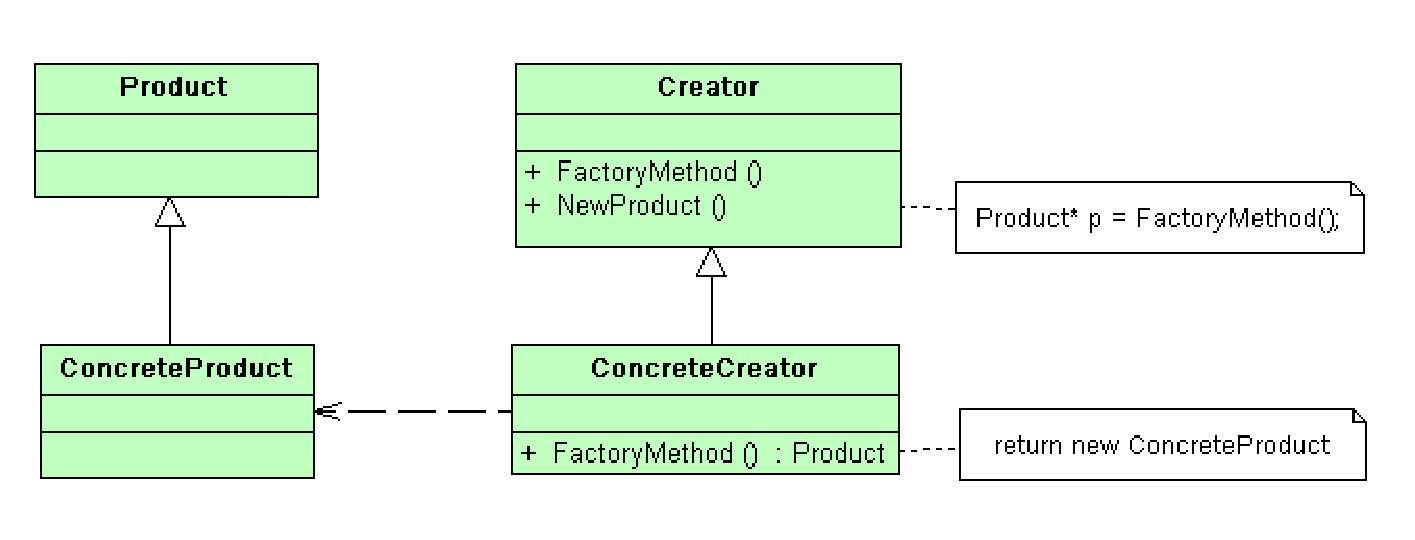
\includegraphics[width=0.9\linewidth]{architech}}
\caption{Основной алгоритм}
\label{architech:architech}
\end{figure}

Использование данного шаблона позволило нам разбить наш проект на независимые модули, что весьма упростило задачу разработки, так как написание алгоритма для конкретного таска не влияло на остальную часть проекта. При разработке был реализован базовый класс для работы с образом диска. Данный клас предназначался для формирования списка настроек, определения операционной системы на смонтированном образе и инстанционировании и накапливание всех необходимых классов-тасков в очереди тасков. После чего каждый таск из очереди отправлялся на выполнение. Блоксхема работы алгоритма (тут картинка alg_main.eps)

Каждый класс-таск порождался путем наследования от базового абстрактного класса который имеет 8 методов и 3 атрибута:

\begin{enumerate}
\item QString manual() - возвращает справку о входных параметрах данного таска;
\item void setOption(QStringList list) - установка флагов для поданных на вход параметров;
\item QString command() - возвращает команду для инициализации такска вручную;
\item bool supportOS(const coex::typeOS \&os) - возвращает флаг, указывающий на возможность использования данного таска для конкретной операционной системы;
\item QString name() - возвращает имя данного таска;
\item QString description() - возвращает краткое описание таска;
\item bool test() - предназначена для теста на доступность таска;
\item bool execute(const coex::config \&config) - запуск таска на выполнение;
\item QString m\_strName - хранит имя таска;
\item QString m\_strDescription - хранит описание таска;
\item bool m\_bDebug - флаг для параметра --debug;
\end{enumerate}

На данный момент в проекте используется восемь классов. UML-диаграмма классов представлена на рисунке (тут картинка UML.eps)

Классы taskSearchSyslogsWin, taskSearchPidginWin и taskSearchSkypeWin - наследники от класса task являются тасками. Класс winEventLog и _EVENTLOGRECORD предназначины для конвертации журнальных файлов операционной системы Windows XP, а класс writerMessages для преобразования истории переписки.

\newpage
\subsection{Сбор информации из браузера Google Chrome} % - Отчёт Влада
\input{individual_reports/Shipovskoy}

\newpage
\subsection{Cбор информации из мессенджера ICQ} % - Отчёт Юры
\input{individual_reports/Tereshenko}

\newpage
\subsection{Cбор информации из почтового клиента MS Outlook} % - Отчёт Андрея
\input{individual_reports/Seryakov}

\newpage
\subsection{Идентификации файлов изображений} % - Отчёт Ильи
Целью работы стало написание модуля для программного комплекса. Модуль выполняет проверку файлов-изображений на их подлинность (являются ли они действительно изображением), и выводить информацию в формате XML.

\subsubsection{Реализация программного модуля}
Сначала необходимо было узнать, как различать изображения и файлы с расширением изображений. Было принято решение считывать заголовки файлов и сравнивать их с корректными заголовками, являющимися уникальными для соответствующего формата. Далее была найдена информация о заголовках нескольких форматов. Форматы заголовков представлены в таблице~\ref{tab:formats}.

% таблица форматов заголовков
\begin{table}[ht]
\caption{Форматы заголовков}
\label{tab:formats}
\begin{center}
\begin{tabular}{|p{8cm}|p{9cm}|}
\hline
Формат & Заголовок \\
\hline
JPEG & FFD8 \\
\hline
PNG & 89504E47 \\
\hline
GIF & 474946 \\
\hline
BMP & 424D \\
\hline
TIFF & 49492A \\
\hline
\end{tabular}
\end{center}
\end{table}

Также было принято решение проверять на корректность конец файла, так как к изображению можно прикрепить архив в конец файла. На данный момент реализована проверка конца файла для форматов JPEG и PNG как самых популярных и простых для реализации (табл.~\ref{tab:ends}).

% таблица форматов конца файла
\begin{table}[ht]
\caption{Форматы конца файла}
\label{tab:ends}
\begin{center}
\begin{tabular}{|p{8cm}|p{9cm}|}
\hline
Формат & Конец \\
\hline
JPEG & FFD9 \\
\hline
PNG & AE426082 \\
\hline
\end{tabular}
\end{center}
\end{table}

\subsubsection{Алгоритм работы модуля}
Алгоритм программы, проверяющей заголовки и концы файлов, представлен на рисунке~\ref{block_ilya:block_ilya}.

\begin{figure}[h!]                                          % тут рисунок block_ilya
\center{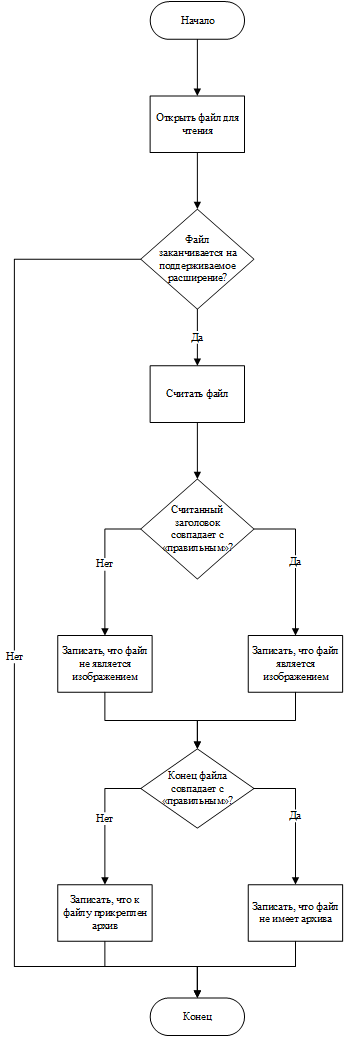
\includegraphics[scale=0.9]{block_ilya}}
\caption{Блок-схема алгоритма программы, проверяющей заголовки и концы файлов}
\label{block_ilya:block_ilya}
\end{figure}

\subsubsection{Структура XML-файла}
Файл начинается с пролога, описывающего версию XML и кодировку. Далее идет начальный элемент <add>, а для каждого изображения создается элемент <doc>. В теле <doc> записаны поля <field name>value</field>, далее закрывается элемент </doc>, а в конце документа находится конечный элемент </add>.

Пример структуры XML-файла представлен на рисунке~\ref{xml_ilya:xml_ilya}.

\begin{figure}[h!]                                          % тут рисунок xml_ilya
\center{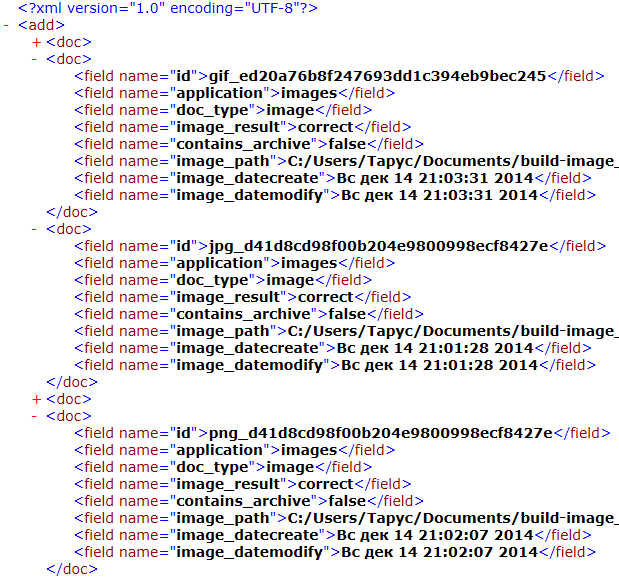
\includegraphics[width=0.6\linewidth]{xml_ilya}}
\caption{Структура XML-файла}
\label{xml_ilya:xml_ilya}
\end{figure}

Значение поля id --- «формат изображения»\_«MD5 сумма от файла».
Поля image\_result и contains\_archive непосредственно указывают на то, является ли файл изображением, и прикреплен ли к нему архив соответственно. Также имеется полный путь до файла, дата создания и дата изменения.
В программу были введены следующие тесты: 5 файлов изображений для базовой проверки, 5 текстовых файлов с расширением изображений, и 2 файла изображений с прикрепленным к ним архивам. Все файлы программа распознала корректно и вывела в XML файл.


Библиотеки Qt, использованные для написания программного модуля:
\begin{itemize}
\item QFile --- для открытия и чтения всего файла;
\item QString --- для работы со строками в программе;
\item QDebug --- для вывода в консоль в целях отладки;
\item QDataStream --- для считывания отдельных байтов из потока;
\item QXmlStreamWriter --- для вывода в XML;
\item QFileInfo --- для считывания информации о файле (даты и т.д.);
\item QDateTime --- для работы с форматом даты, в который записывается информация о файле;
\item QCryptographicHash --- для получение md5 суммы.
\end{itemize}


Результат работы программы представлен на рисунке~\ref{result_ilya:result_ilya}.

\begin{figure}[ht]                                          % тут рисунок result_ilya
% \center{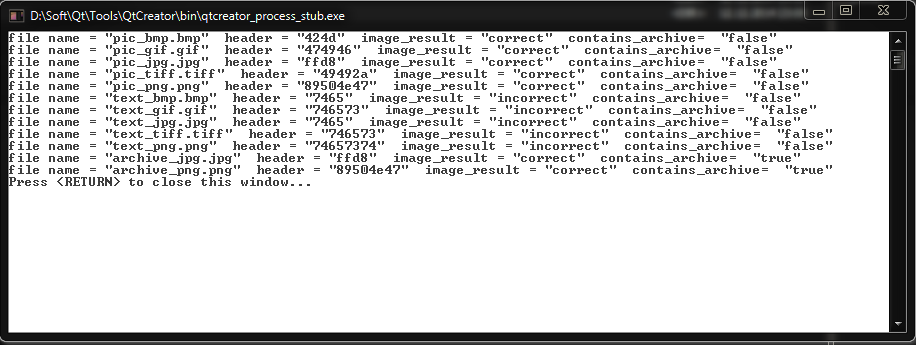
\includegraphics[width=0.6\linewidth]{result_ilya}}
\center{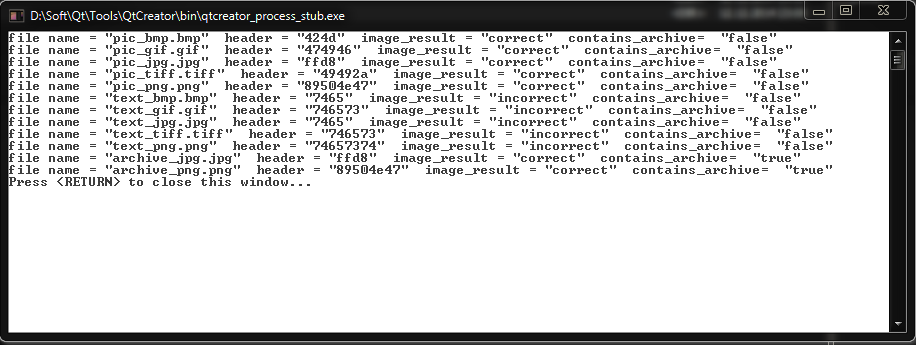
\includegraphics[scale=0.7]{result_ilya}}
\caption{Результат работы программы}
\label{result_ilya:result_ilya}
\end{figure}

\subsubsection{Задачи на следующий семестр}
В будущем в программе будут реализованы:
\begin{itemize}
\item  поддержка новых расширений;
\item  возможность проверить наличие архива для всех расширений;
\item  рекурсивный обход директорий.
\end{itemize}

\clearpage



\newpage 
\subsection{Сбор и анализ информации из реестра ОС MS Windows} % - Отчет Олега
\input{individual_reports/Lobanov}

\newpage 
\subsection{Сбор и анализ информации об установленном ПО по остаточным файлам} % - Отчет Макса
\input{individual_reports/Kucher}

\newpage
\section{Задачи на следующий семестр \textbf{ПРАВИТЬ!!!}}
\begin{enumerate}
\item тестирование системы;
\item подготовка deb-пакета, лицензии;
\item написание публикации.
\end{enumerate}


\newpage
\section*{Заключение}
\addcontentsline{toc}{section}{Заключение}
В данном семестре нашей группой была выполнена часть работы по созданию автоматизированного программного комплекса для проведения компьютерной экспертизы, проанализированы дальнейшие перспективы и поставлены цели для дальнейшего развития проекта.
 
 
 \newpage
 \renewcommand{\refname}{Список использованных источников}
 \bibliography{lit}

 \ESKDappendix{Обязательное}{\normalfont Компакт-диск}
 Компакт-диск содержит: 
 \begin{itemize}
 \item электронную версию пояснительной записки в форматах *.tex и *.pdf;
 \item актуальную версию программного комплекса для проведения компьютерной экспертизы;
 \item тестовые данные для работы с программным комплексом.
 \end{itemize}
 
\end{document}
